\documentclass[12pt]{article}
\usepackage[utf8]{inputenc}
\usepackage[english]{babel}
% \usepackage{titling}
% \usepackage{fancyhdr}
% \usepackage{amssymb,amsmath,amsthm}
\usepackage{geometry}
% \usepackage{layouts}
\usepackage{listings} % for code snippets
\usepackage{xcolor}
\usepackage{graphicx}
\usepackage{titlesec}
% \usepackage{tabularx}

% page setup and spacing
\geometry{a4paper, margin=0.75in}
\setlength{\parindent}{1em}
\setlength{\parskip}{1em}
\renewcommand{\baselinestretch}{1.0}

% \titleformat{\subsection}[display]
% {\normalfont\large\bfseries}
% {\thesection}{}{}

\titlespacing{\subsection}
{0.1pt}{0.1pt}{0.1pt}


% colors for code snippet
\definecolor{codegreen}{rgb}{0,0.6,0}
\definecolor{codegray}{rgb}{0.5,0.5,0.5}
\definecolor{codepurple}{rgb}{0.58,0,0.82}
\definecolor{backcolour}{rgb}{0.95,0.95,0.92}

% code snippet styling
\lstdefinestyle{mystyle}{
    backgroundcolor=\color{backcolour},   
    commentstyle=\color{codegreen},
    keywordstyle=\color{magenta},
    numberstyle=\tiny\color{codegray},
    stringstyle=\color{codepurple},
    basicstyle=\ttfamily\footnotesize,
    breakatwhitespace=false,         
    breaklines=true,                 
    captionpos=b,                    
    keepspaces=true,                 
    numbers=left,                    
    numbersep=5pt,                  
    showspaces=false,                
    showstringspaces=false,
    showtabs=false,                  
    tabsize=2
}
\lstset{style=mystyle}

\title{ESOF 322: Homework 2}
\author{River Kelly}
\date{September 21, 2021}

\begin{document}

\maketitle
\begin{center}
Partner: Peyton Dorsh    
\end{center}

\newpage

\section*{Exercise Part A (15 pts)}
\subsection*{1. (2pts)}
\includegraphics[width=\textwidth]{HW-2-diagrams-Part-A-1.png}
\subsection*{2. (3pts)}
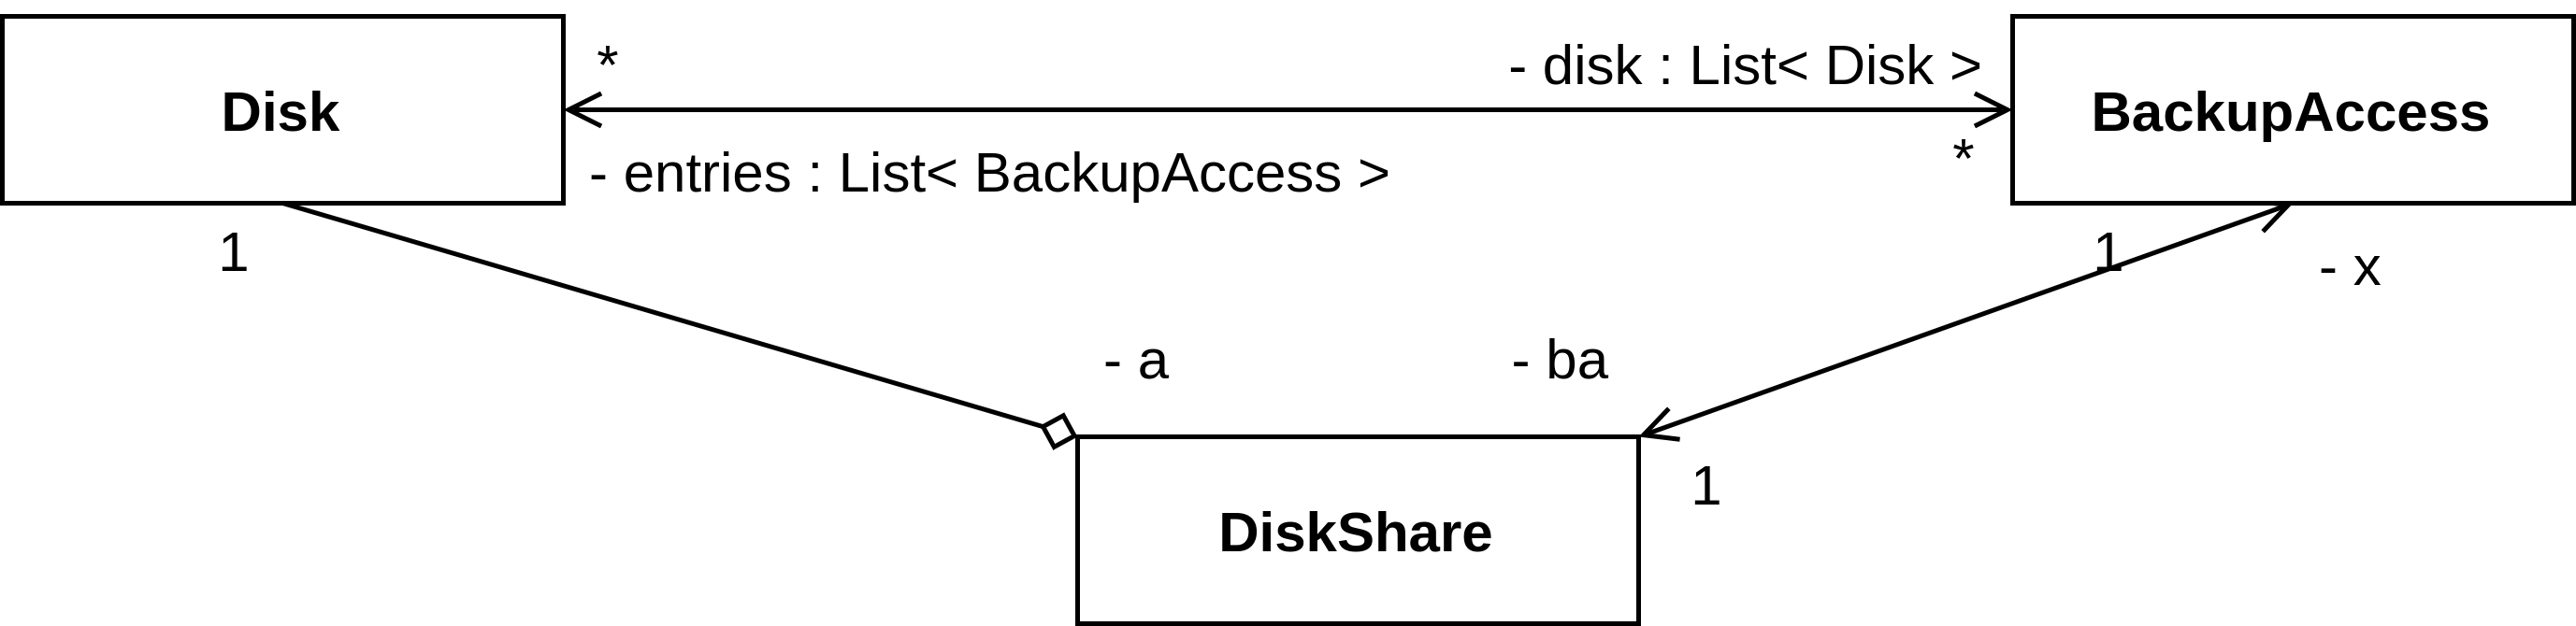
\includegraphics[width=\textwidth]{HW-2-diagrams-Part-A-2.png}
\subsection*{3. (5pts)}
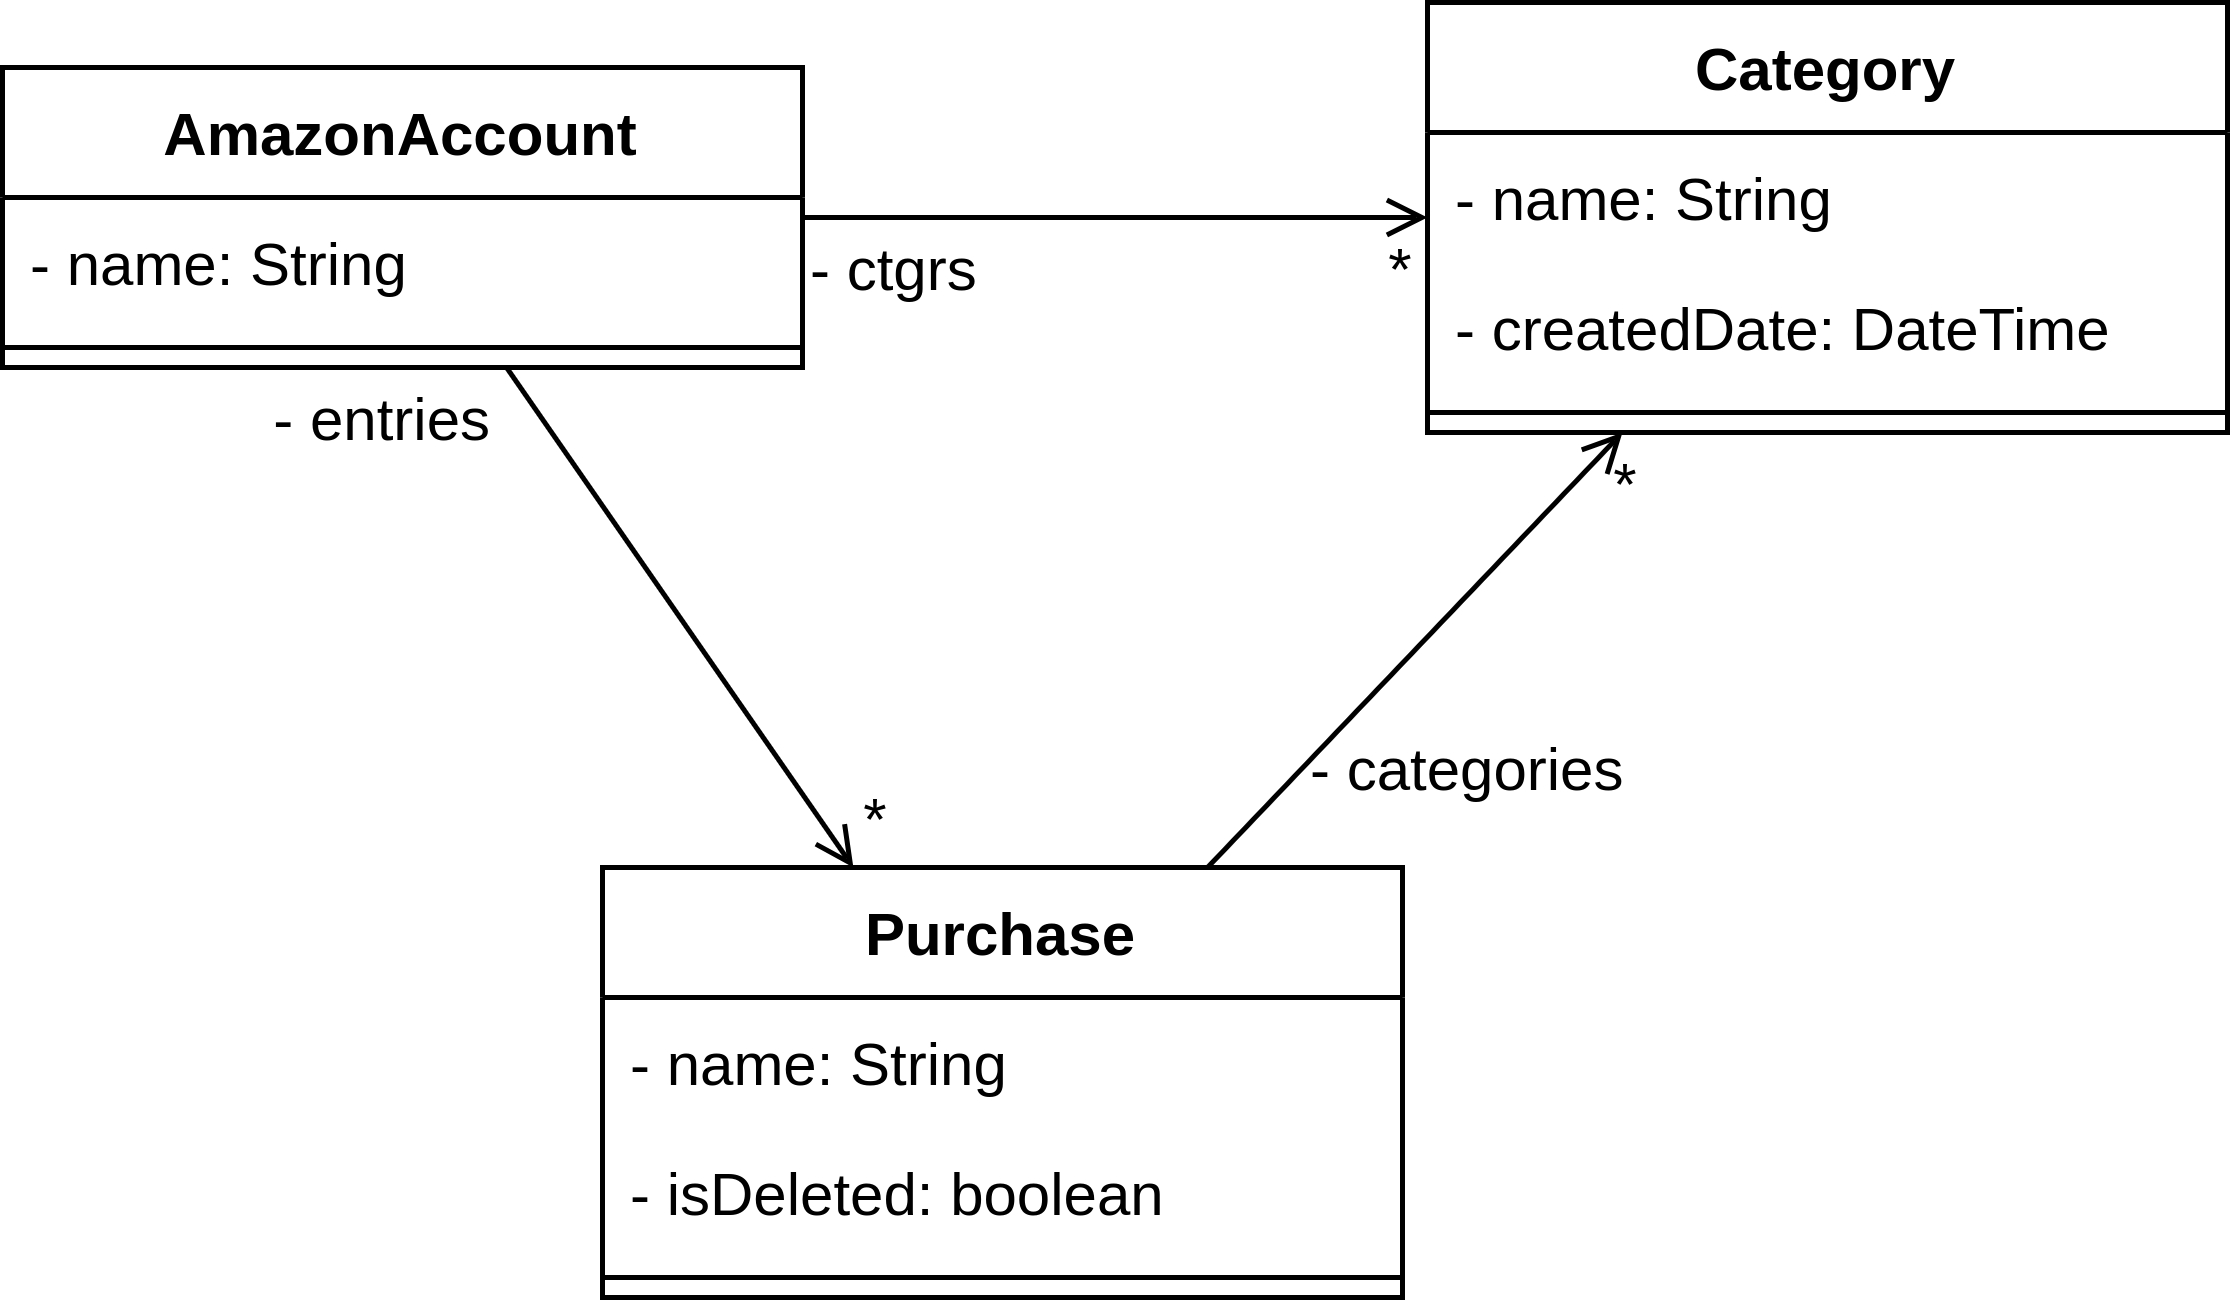
\includegraphics[width=\textwidth]{HW-2-diagrams-Part-A-3.png}
\subsection*{4. (5pts)}
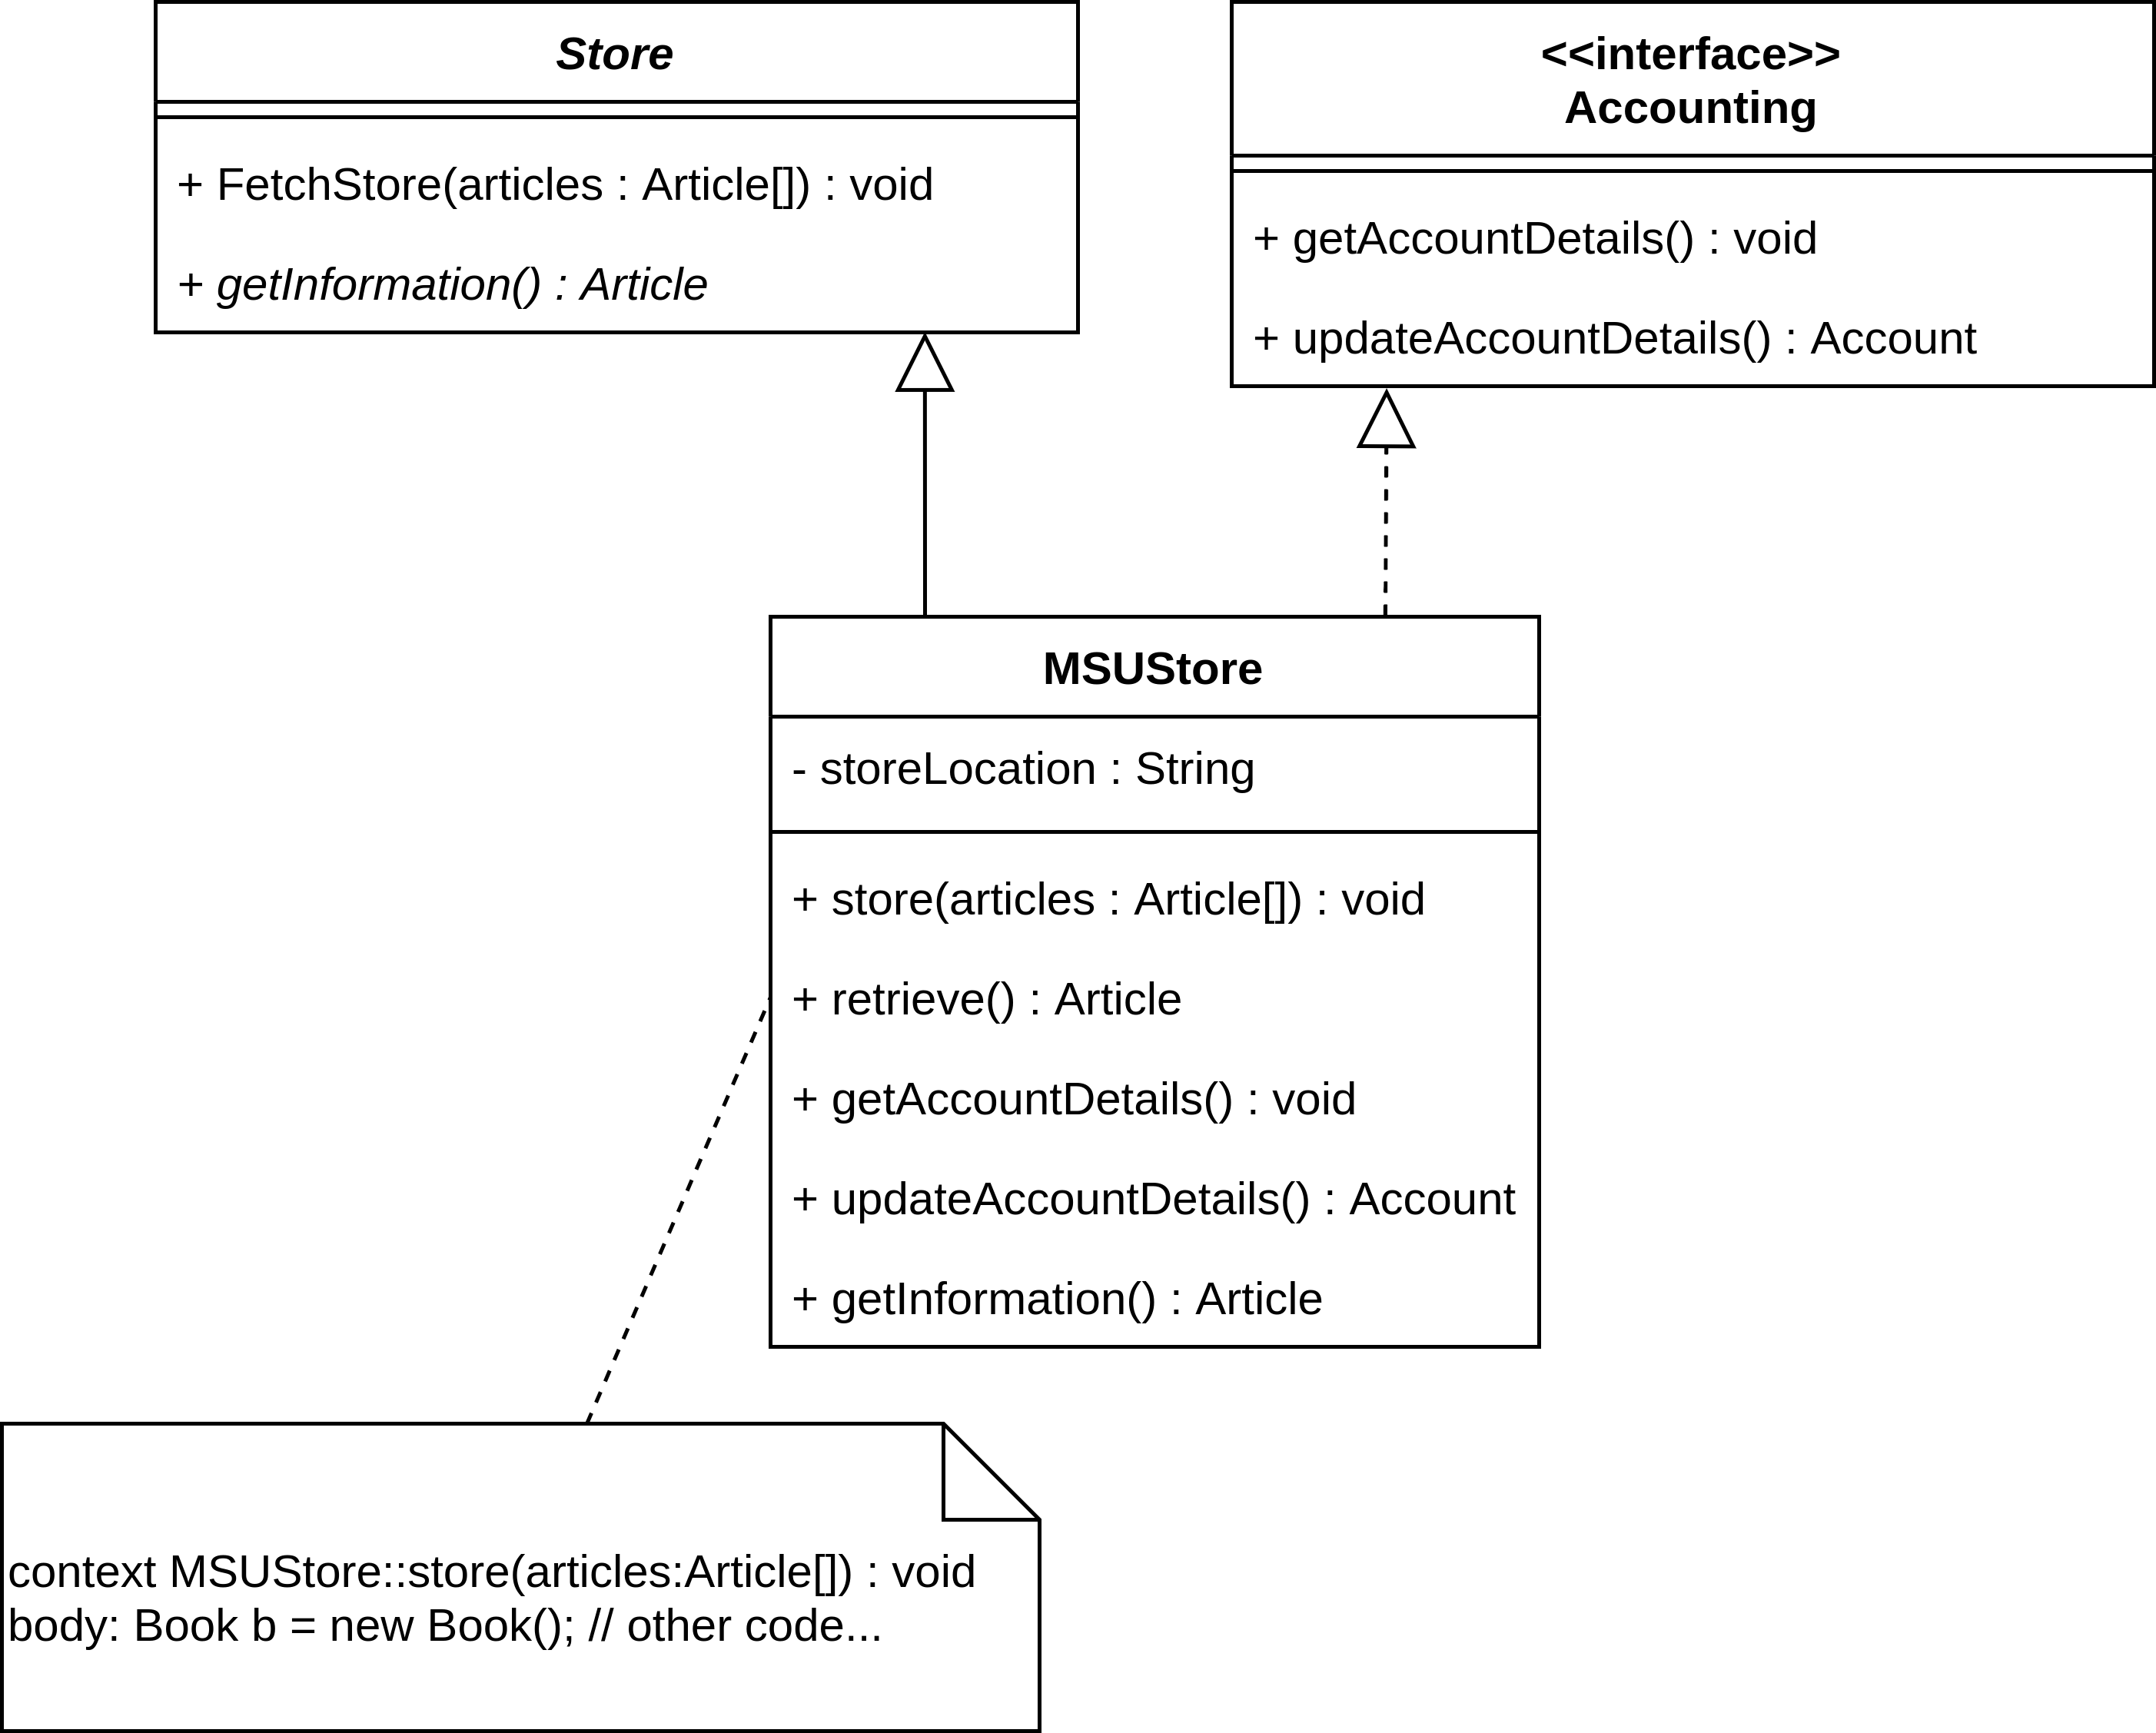
\includegraphics[width=\textwidth]{HW-2-diagrams-Part-A-4.png}

\newpage

\section*{Exercise Part B (15 pts)}

Write \textbf{pseudo code} to describe the following UML class diagram:

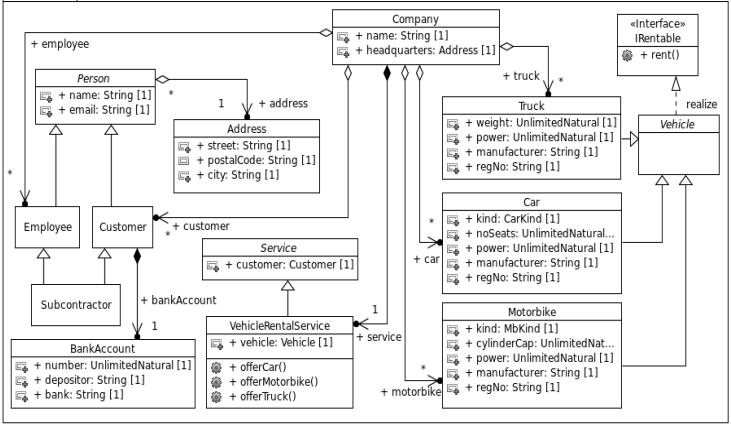
\includegraphics[width=\textwidth]{HW-2-B-image.png}
\subsection*{Company Class}
% Company Class
\begin{lstlisting}[language=Java]
public class Company {
  public String name;
  public Address headquarters;
  
  // properties from associations
  public Customer customer;
  public Employee employee;
  public VehicleRentalService service;
  public Truck truck;
  public Car car;
  public Motorbike motorbike;

  // Company Destructor
  public void finalize() {
    delete service (this.service)
    delete self (delete this)
  }
}
\end{lstlisting}

% Service
\subsection*{Service Class}
\begin{lstlisting}[language=Java]
public abstract class Service {
    public Customer customer;
}
\end{lstlisting}

\newpage
% VehicleRentalService
\subsection*{VehicleRentalService Class}
\begin{lstlisting}[language=Java]
public abstract class VehicleRentalService {
    public Vehicle vehicle;
    public offerCar();
    public offerMotorbike();
    public offerTruck();
}
\end{lstlisting}


\subsection*{IRentable Class}
% IRentable
\begin{lstlisting}[language=Java]
public interface IRentable {
  public void rent() {}
}
\end{lstlisting}


\subsection*{Vehicle Class}
% Vehicle
\begin{lstlisting}[language=Java]
public class Vehicle implements IRentable {
  public UnlimitedNatural power;
  public String manufacturer;
  public String regNo;

  public void rent() {
    some code to rent the vehicle
  }
}
\end{lstlisting}
\subsection*{Truck Class}
% Truck
\begin{lstlisting}[language=Java]
public class Truck extends Vehicle {
  public UnlimitedNatural weight;
}
\end{lstlisting}
\subsection*{Car Class}
% Car
\begin{lstlisting}[language=Java]
public class Car extends Vehicle {
  public CarKind kind;
  public UnlimitedNatural noSeats;
}
\end{lstlisting}
\subsection*{Motorbike Class}
% Motorbike
\begin{lstlisting}[language=Java]
public class Motorbike extends Vehicle {
  public MbKind kind;
  public UnlimitedNatural cylinderCap;
}
\end{lstlisting}
\subsection*{Person Class}
% Person
\begin{lstlisting}[language=Java]
public class Person {
  public String name;
  public String email;
  // properties from associations
  public Address address;
}
\end{lstlisting}
\subsection*{Address Class}
% Address
\begin{lstlisting}[language=Java]
public class Address {
  public String street;
  public String postalCode;
  public String city;
}
\end{lstlisting}
\subsection*{Customer Class}
% Customer
\begin{lstlisting}[language=Java]
public class Customer extends Person {
  
  // properties from associations
  public BankAccount bankAccount;

  // Customer Destructor
  public void finalize() {
    delete bank account (this.bankAccount)
    delete self (delete this)
  }

}
\end{lstlisting}
\subsection*{Employee Class}
% Employee
\begin{lstlisting}[language=Java]
public class Employee extends Person {}
\end{lstlisting}
\subsection*{Subcontractor Class}
% Subcontractor
\begin{lstlisting}[language=Java]
public class Subcontractor extends Person, Employee {}
\end{lstlisting}
\subsection*{BankAccount Class}
% BankAccount
\begin{lstlisting}[language=Java]
public class BankAccount {
  public UnlimitedNatural number;
  public String depositor;
  public String bank;
}
\end{lstlisting}
\newpage

\section*{Exercise Part C (5 pts)}

\textbf{Suppose we need to develop a system named ‘Retail System’. Draw a single use case diagram capturing the following 4 use cases.}

\begin{itemize}
    \item A manager can add a new product in the system.
    \item A manager can delete a product in the system.
    \item A manager can edit a product information in the system.
    \item Both use cases (i), (ii) and (iii) should reuse this new use case i.e., a product should be available in the stock.
\end{itemize}

\begin{center}
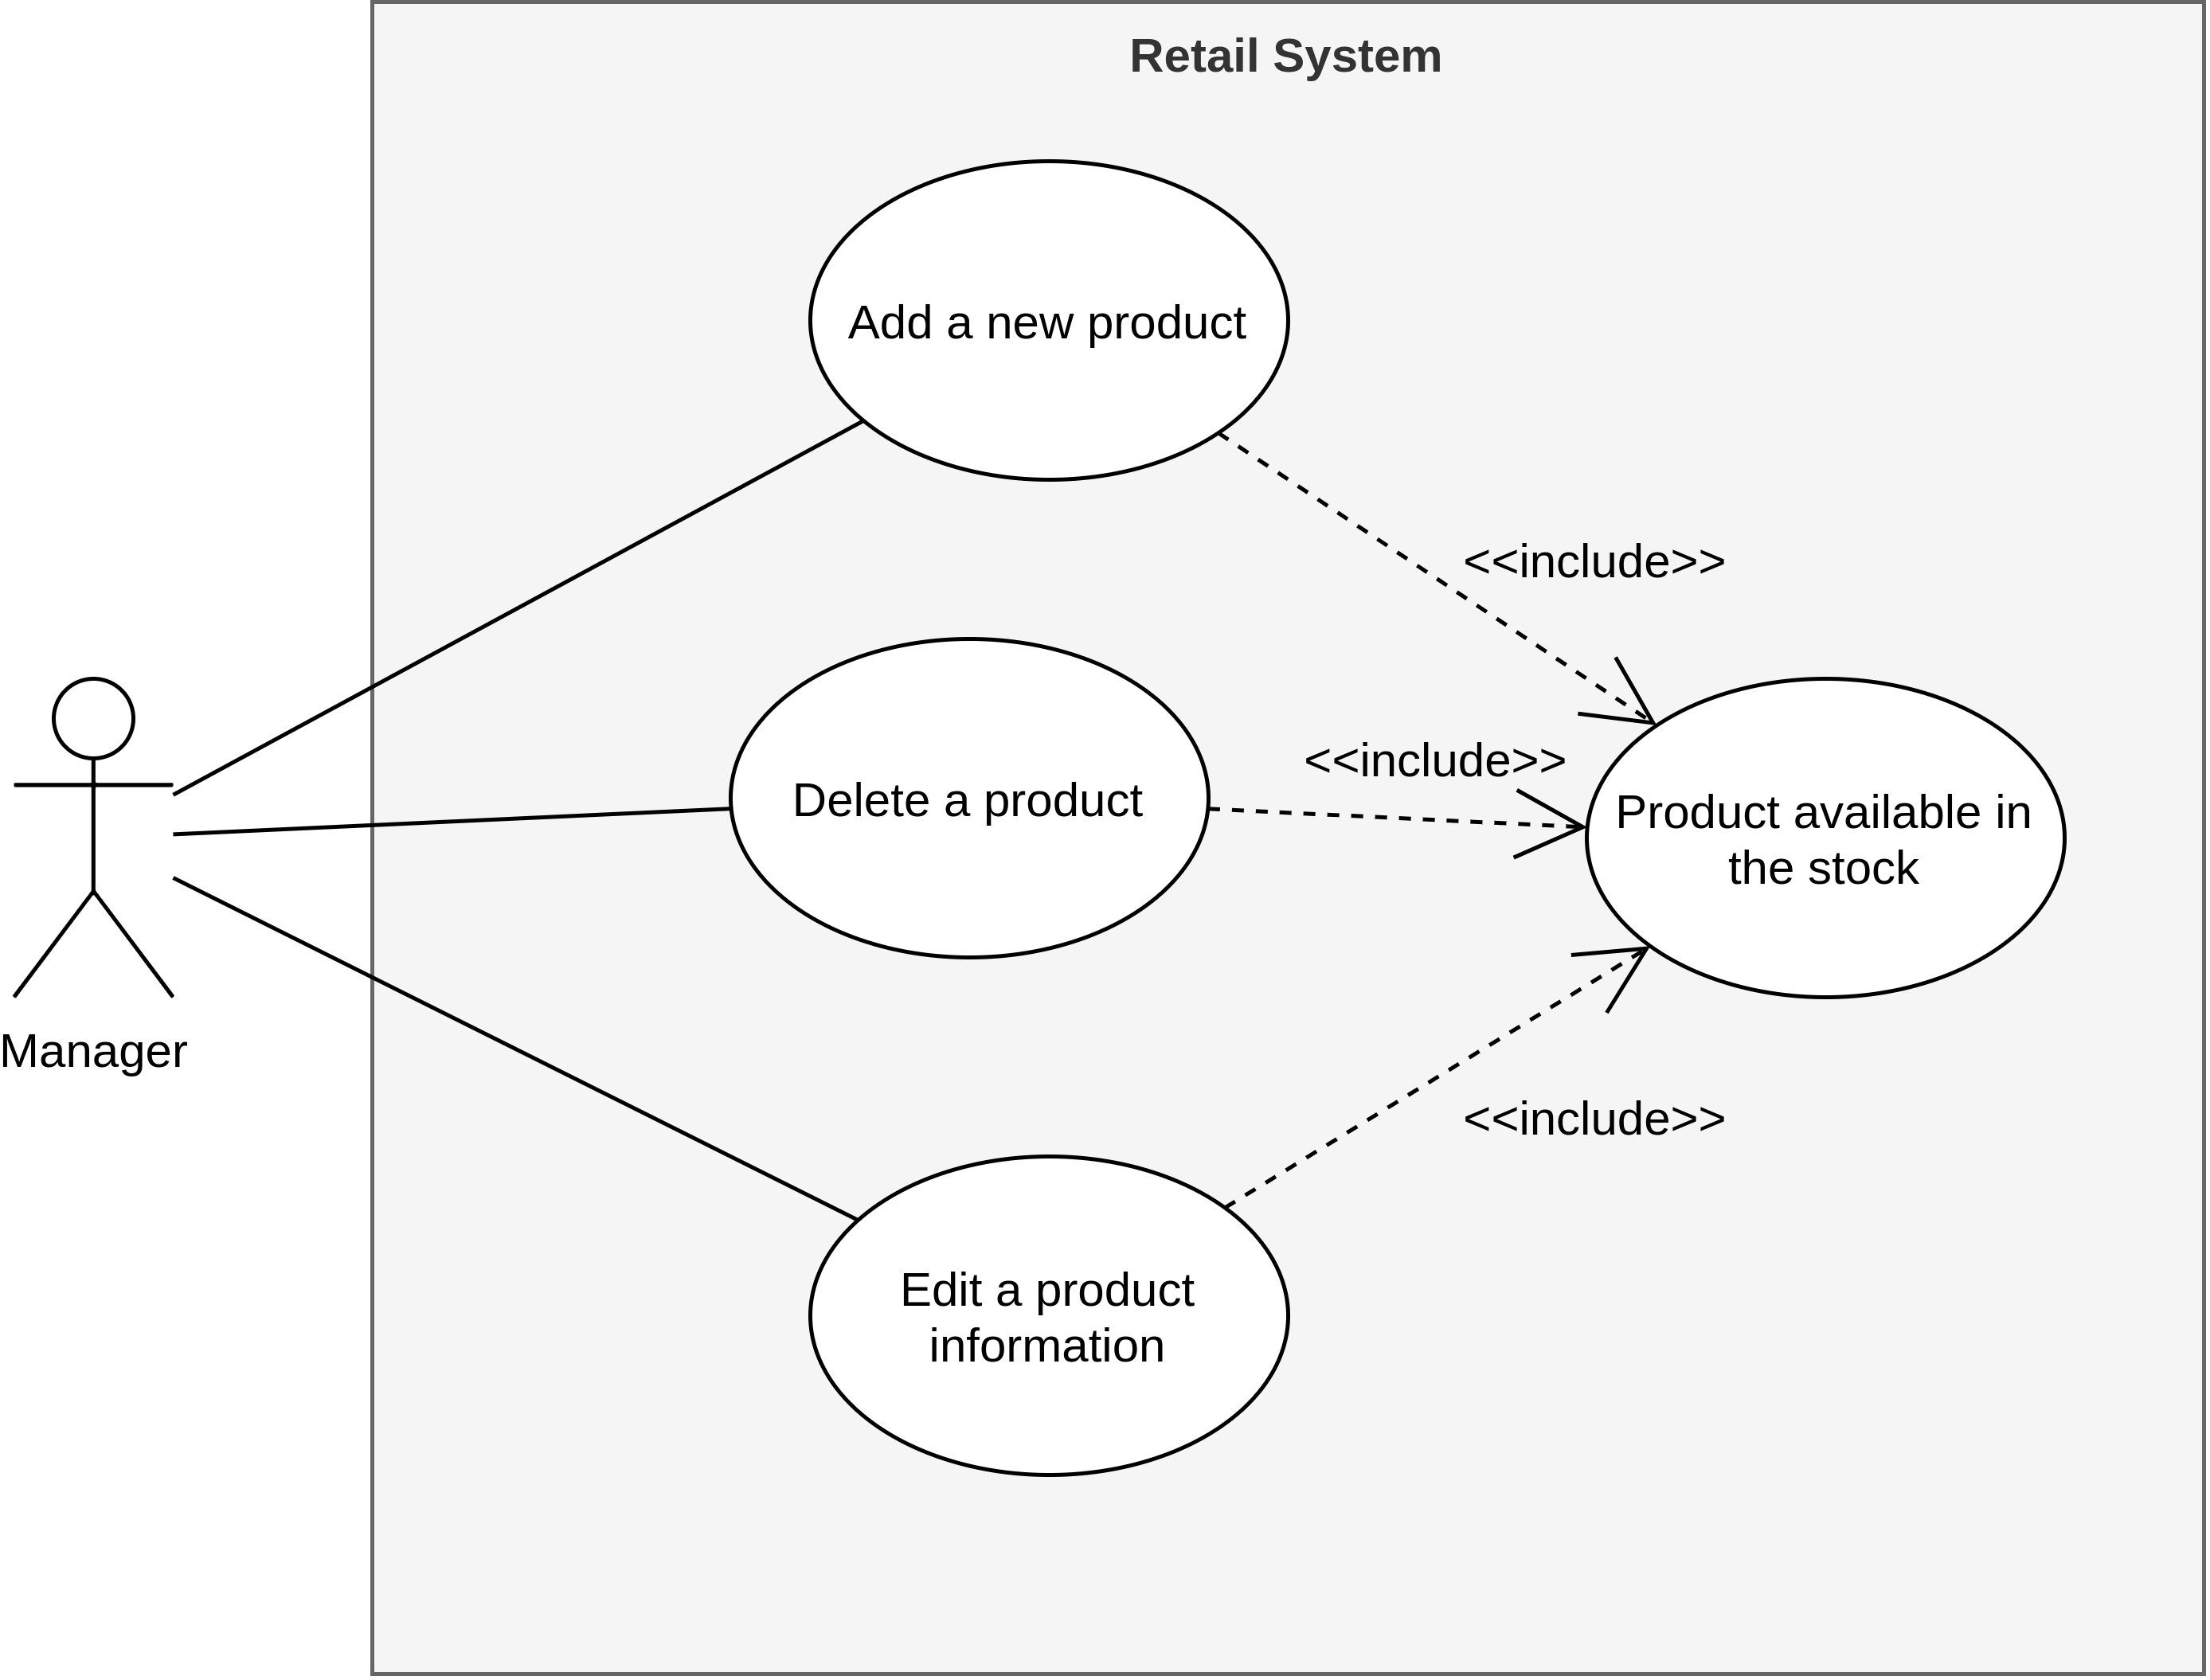
\includegraphics[width=0.5\textwidth]{HW-2-diagrams-Part-C.png}
\end{center}

\subsection*{Use Case: Add a new Product}
\begin{center}
\begin{tabular}{ l p{0.65\textwidth} }
    \textbf{Use case name}: & Add a new Product \\
    % \textbf{Related Requirements}: & Requirement 1 \\
    \textbf{Goal In Content}: & A Manager requests to create and add a new product to the store inventory \\
    \textbf{Preconditions}: & Check if a duplicate product already exists in the Store inventory \\
    \textbf{Successful End Condition}: & A new product is added to the store inventory \\
    \textbf{Failed End Condition}: & The request for creating a new Product in the store’s inventory is rejected  \\
    \textbf{Primary Actors}: & Manager  \\
    % \textbf{Secondary Actors}: & Member Credentials Database  \\
    \textbf{Trigger}: & The Manager asks the Retail Store to create a new product  \\
    \textbf{Main Flow}: & 1. The Manager requests the Retail Store to create a new product\newline 2. See if product is already available (i.e. if it is a duplicate)\newline 3. The new product is created \newline 4. The product is available in the store’s inventory\\
\end{tabular}
\end{center}

\subsection*{Use Case: Delete a Product in the system}
\begin{center}
\begin{tabular}{ l p{0.65\textwidth} }
    \textbf{Use case name}: & Delete a product in the system \\
    % \textbf{Related Requirements}: & Requirement 1 \\
    \textbf{Goal In Content}: & A Manager requests to remove an existing product from the store’s inventory \\
    \textbf{Preconditions}: & The product must exist in the store’s inventory \\
    \textbf{Successful End Condition}: & The product is deleted from the store’s inventory \\
    \textbf{Failed End Condition}: & The product is not removed from the store’s inventory  \\
    \textbf{Primary Actors}: & Manager  \\
    % \textbf{Secondary Actors}: & Member Credentials Database  \\
    \textbf{Trigger}: & The Manager asks the Retail Store to delete a product  \\
    \textbf{Main Flow}: & 1. The Manager makes a request to the Retail Store to remove a product\newline 2. The systems checks if the product exists in the store’s inventory\newline 3. The product is removed from the store’s inventory
\end{tabular}
\end{center}

\subsection*{Use Case: Edit product information}
\begin{center}
\begin{tabular}{ l p{0.65\textwidth} }
    \textbf{Use case name}: & Edit a product’s information in the system \\
    % \textbf{Related Requirements}: & Requirement 1 \\
    \textbf{Goal In Content}: & A Manager requests to update the information of an existing product in the store’s inventory \\
    \textbf{Preconditions}: & The product must exist in the store’s inventory \\
    \textbf{Successful End Condition}: & The product’s information is updated in the system \\
    \textbf{Failed End Condition}: & The product’s information is not updated  \\
    \textbf{Primary Actors}: & Manager  \\
    % \textbf{Secondary Actors}: & Member Credentials Database  \\
    \textbf{Trigger}: & The Manager asks the Retail Store to update a product’s information  \\
    \textbf{Main Flow}: & 1. The Manager makes a request to the Retail Store to update a product’s information\newline 2. The systems checks if the product exists in the store’s inventory\newline 3. The product’s information is updated in the system
\end{tabular}
\end{center}

\subsection*{Use Case: A product should be available in the stock}
\begin{center}
\begin{tabular}{ l p{0.65\textwidth} }
    \textbf{Use case name}: & A product should be available in the stock \\
    % \textbf{Related Requirements}: & Requirement 1 \\
    \textbf{Goal In Content}: & The existence of a product in the system is checked \\
    % \textbf{Preconditions}: & The product must exist in the store’s inventory \\
    \textbf{Successful End Condition}: & The product is in stock \\
    \textbf{Failed End Condition}: & The product is not in stock \\
    \textbf{Primary Actors}: & Manager  \\
    % \textbf{Secondary Actors}: & Member Credentials Database  \\
    \textbf{Trigger}: & A request to update an item in the store’s inventory is made  \\
    \textbf{Main Flow}: & 1. A Manager requests to make some update to the store’s inventory\newline 2. The systems checks if the product is in stock
\end{tabular}
\end{center}

\end{document}
